\documentclass[10pt,a4paper]{article}
\usepackage[utf8]{inputenc}
\usepackage[T1]{fontenc}
\usepackage{amsmath,amssymb,amsfonts}
\usepackage{graphicx}
\usepackage{hyperref}
\usepackage{algorithm}
\usepackage{algpseudocode}
\usepackage{booktabs}
\usepackage{lipsum}
\usepackage{geometry}
\usepackage{cite}
\usepackage{authblk}
\usepackage{mathtools, empheq}
\usepackage{multicol}
\usepackage{tikz}
\usetikzlibrary{arrows.meta, positioning, shapes.geometric}
\geometry{margin=2cm}
\title{Simulating the End of Work and Money: A Microsimulation of AGI-Driven Automation}
\author{\large Fabien Furfaro\thanks{\texttt{fabien.furfaro@gmail.com}}}
\date{\large 2025}

% ------------------------------------------------------------------------
% Style Reminder Helper (For AI Assistant): Keep every sentence in abstracts and main text neutral, humble, and scientific.
% Write in ENGLISH only
% For each sentence, check for "marketing" tone (e.g., overuse of words like "novel", "substantial", "robust") or subjective point of view (e.g., "traditionnal", "essential")
% and replace with more cautious, evidence-based claims.
%
% Prefer:
% - "show", "suggest", "may improve", "offers potential", "addresses some limitations"
% - "To the best of our knowledge...", "Preliminary experiments suggest...",
%   "Further investigation is needed...", "This approach may be of interest..."
%
% Apply rules : Less is More
% Avoid:
% - "groundbreaking", "revolutionary", "unprecedented", "definitively demonstrates",
%   overly strong claims without empirical or theoretical backing
%
% Make explicit:
% - Limitations, resource constraints, preliminary or ongoing nature of results,
%   encouragement for community replication and extension.
% Example sentences:
% - "We propose a novel architecture..." → "We propose an alternative architecture..."
% - "Substantially improves..." → "Shows promising results..." / "May improve..."
% - "Our approach is fully robust..." → "Preliminary results suggest some robustness..."
%
% Always use conditional language ("could", "might", "suggests") when appropriate and prefer cautious claims.
% Before finalizing, review each sentence with these criteria in mind.

% Structure IMRaD 
% ------------------------------------------------------------------------

\begin{document}
\maketitle

\begin{abstract}
The development of Artificial General Intelligence (AGI) raises fundamental questions about the transformation of labor markets through widespread task automation at declining marginal costs. This paper presents a microsimulation framework modeling firm-level automation decisions as a repeated non-cooperative game, structurally analogous to the Prisoner's Dilemma. Within this framework, firms iteratively adjust their automation levels to maximize profits, balancing competitive advantages from out-automating rivals against implementation costs.

The model explores how varying competitive pressures, baseline automation gains, and cost structures influence long-term equilibrium outcomes. Simulations suggest that automation adoption patterns are highly context-dependent: competitive incentives may drive substantial labor substitution under certain conditions, while cost constraints can limit automation even in competitive environments.

These dynamics highlight potential risks of wage-based demand collapse and challenge the sustainability of traditional labor markets in an AGI-driven economy. The findings also point to possible policy responses, such as automation taxation or universal basic income mechanisms funded by AI-generated rents, to mitigate adverse economic and social consequences.
\end{abstract}

\section{Introduction}
\label{sec:introduction}

The rapid advancement of Artificial General Intelligence (AGI) has sparked discussions about its potential to reshape labor markets by automating cognitive and physical tasks at declining marginal costs \cite{acemoglu2025simple,goertzel2014artificial}. This transformation carries economic implications, including possible productivity gains alongside risks of labor displacement. Observed disparities in AI adoption across regions suggest that uneven labor market impacts may arise, particularly where worker adaptation lags behind technological change \cite{cerutti2025global,filippucci2025macroeconomic}. Recent scenario-based methodologies highlight the heterogeneity of AGI's societal impacts across regions and sectors \cite{costa2025exploring}.

\subsection{Context: AGI and the Future of Labor}
Empirical and theoretical work indicates that automation has historically displaced routine tasks while complementing non-routine cognitive activities—a pattern that AGI's general capabilities might alter \cite{autor2015there}. Macroeconomic analyses suggest that AI-induced task substitution could reduce labor shares, partially offset by the creation of new tasks \cite{acemoglu2025simple}. However, models such as the Constant Elasticity of Substitution (CES) framework predict more dramatic shifts, where accelerated capital-labor substitution under AGI could lead to employment declines in certain sectors \cite{stiefenhofer2025future,gondauri2025impact}. Recent work on endogenous automation and task creation suggests that competitive firm interactions may lead to socially inefficient outcomes, such as excessive labor substitution or misallocation of resources \cite{martinez2018automation}.

\subsection{Research Problem and Contribution}
This study examines the following question: \textit{How do competitive dynamics between firms influence automation adoption, and what are the potential consequences for labor market equilibria?} The paper contributes to the literature by:
\begin{itemize}
    \item Modeling firm-level automation decisions as a non-cooperative game, with structural parallels to the Prisoner's Dilemma, to isolate the role of competitive pressure and implementation costs.
    \item Simulating automation adoption across a range of parameters, showing that outcomes depend on the interplay between competitive incentives and cost structures.
    \item Discussing potential policy responses, such as automation taxation or universal basic income (UBI) mechanisms, while acknowledging the exploratory nature of these findings.
\end{itemize}


Preliminary results suggest that automation adoption is highly context-dependent: high competitive pressure drives near-complete automation, while elevated costs preserve partial labor substitution \cite{acemoglu2025simple}. These dynamics highlight the potential for wage-demand collapse in the absence of coordination, motivating policy instruments such as automation taxation \cite{filippucci2025macroeconomic} or universal basic income funded by AI rents \cite{schatten2025universal, nayebi2025ai}.


\section{Theoretical Framework: A Non-Cooperative Game of AGI-Driven Automation}
\label{sec:theory}

\subsection{Definition of AGI and Key Assumptions}
Artificial General Intelligence (AGI) refers to hypothetical AI systems capable of matching or exceeding human performance across most economically relevant tasks, including cognitive and physical adaptability \cite{goertzel2014artificial,bostrom2014paths}. Unlike narrow AI, AGI is characterized by cross-domain competence, autonomous improvement, and the ability to substitute for both cognitive and physical labor. By this definition, even the new tasks (eg. creative destruction) could also be replaced by the AGI. This ability to replace human tasks across a wide range of activities provides the basis for modeling automation as a continuous process in the subsequent framework.


\subsection{Comparison of Modeling Approaches}
\label{subsec:comparison}

Empirical evidence indicates that automation has historically displaced routine tasks while complementing non-routine cognitive work—a pattern that AGI's general capabilities could reverse \cite{autor2015there}. While this study focuses on a static, game-theoretic framework to model firm-level automation decisions, alternative approaches exist to capture additional dimensions of AGI adoption. Network effect models \cite{katz1985network,eisenmann2011platform} highlight how firms' automation choices may depend on the decisions of competitors or partners, as seen in the adoption of shared technological standards (e.g., robotic operating systems). Similarly, real options frameworks \cite{dixit1994investment,goertzel2014artificial} emphasize the role of uncertainty in delaying or accelerating automation investments, particularly for irreversible technologies like AGI. These approaches complement our analysis by addressing dynamic interdependencies and strategic timing, which are critical for long-term policy design. Agent-based simulations have shown how micro-level firm behaviors can generate emergent macroeconomic phenomena, including the rise of AI agent economies \cite{glielmo2025beforeit,hadfield2025economy}. These studies underscore the importance of modeling firm-level decision-making to understand aggregate outcomes. To contextualize our framework, we compare it with alternative approaches for modeling AGI-driven automation. Table~\ref{tab:approaches} summarizes their strengths, limitations, and relevance to AGI.

\begin{table}[ht]
\centering
\caption{Comparison of Modeling Approaches for AGI-Driven Automation}
\label{tab:approaches}
\begin{tabular}{@{}p{5cm}p{5cm}p{5cm}@{}}
\toprule
\textbf{Approach}               & \textbf{Strengths}                          & \textbf{Limitations}                     \\
\midrule
CES Production Functions        & Simple, macro-level insights                & No strategic firm behavior               \\
Network Models                  & Captures interdependencies                 & High complexity, data-intensive         \\
Real Options                    & Handles uncertainty and irreversibility    & Static competitive environment           \\
World3/Dynamic Systems          & Endogenous feedback loops, systemic view    & No firm-level strategic interaction      \\
Agent-Based Models              & Heterogeneous agents, emergent phenomena   & Computationally intensive                \\
\textbf{Our Game-Theoretic Model} & \textbf{Firm-level strategies, clear policy levers} & \textbf{Homogeneous firms, static} \\
\bottomrule
\end{tabular}
\end{table}


Macroeconomic frameworks such as World3 simulate system dynamics through differential equations, where population ($P$), capital ($K$), and resources ($R$) interact without explicit strategic firm behavior \cite{meadows2012limits,sterman1980effect}. Our model bridges this gap by focusing on micro-level competition as the driver of automation, generating macro-level labor displacement as an emergent outcome.

We adopt a static, game-theoretic framework for three key reasons: (1) \textbf{parsimony}, as it isolates the core strategic interaction between firms; (2) \textbf{generality}, since equilibrium outcomes are robust to temporal assumptions; and (3) \textbf{policy relevance}, as it directly highlights levers like competition regulation ($\gamma$) or cost manipulation ($k$). While dynamic or network-based approaches \cite{dixit1994investment,katz1985network} could capture additional complexities, our focus on static equilibria provides a clear baseline for understanding the fundamental trade-offs of AGI-driven automation.

This study contributes to the literature by modeling firm automation decisions as a repeated non-cooperative game, structurally analogous to the Prisoner's Dilemma. In this framework, unilateral automation yields a temporary competitive advantage, but collective adoption risks labor displacement and potential demand collapse \cite{stiefenhofer2025artificial}. Unlike aggregate CES frameworks \cite{stiefenhofer2025future,gondauri2025impact}, our microsimulation examines iterative profit maximization across a grid of parameters, including competitive pressure, baseline automation gains, and implementation costs. The model explicitly captures the tension between short-term competitive incentives and long-term systemic risks.


\subsection{Profit Function and Cournot-Nash Equilibrium}

Standard microeconomic theory posits that firms maximize profits \(\Pi_i = R_i - C_i\), where \(\Pi_i\) denotes the profit of firm \(i\), \(R_i\) its revenue, and \(C_i\) its costs. In constrained optimization settings, firms may instead maximize a utility function \(U_i(x_i)\) subject to resource constraints \(\sum x_i \leq \omega\), where \(U_i\) represents the firm's objective (e.g., profit, market share, or a combination of economic outcomes), and \(\omega\) is the total available resource budget \cite{varian1992microeconomic}. The Pareto optimum requires equal marginal utilities across agents:
\[
\frac{\partial U_i}{\partial x_i} = \frac{\partial U_j}{\partial x_j} = \lambda \quad \forall i,j,
\]
a condition that abstracts from dynamic interactions and strategic behavior \cite{arrow2024existence}. While general equilibrium models capture resource allocation, they typically overlook the iterative, competitive processes driving firm-level decisions in oligopolistic markets. To analyze how firms adjust their automation strategies in response to competitive pressures, we adopt a game-theoretic framework based on the following assumptions:
\begin{itemize}
    \item Firms operate in an oligopolistic market where automation decisions are strategic complements, meaning each firm's choice directly affects the profitability of its rivals.
    \item Automation is modeled as a continuous variable \(a_i \in [0,1]\), representing the fraction of tasks automated by firm \(i\).
    \item Firms aim to maximize profits, balancing the benefits of automation (competitive advantage, cost savings) against its associated costs (implementation, disruption).
\end{itemize}



% --- Figures ---
\begin{figure}[ht]
    \centering
    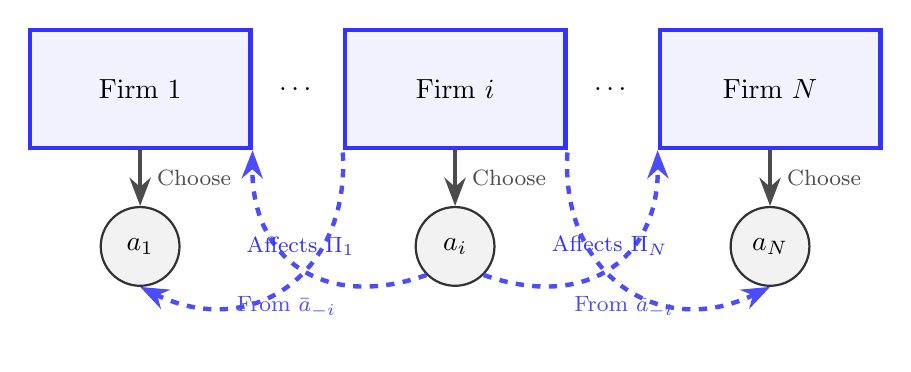
\begin{tikzpicture}[
        % STYLES
        firm/.style={rectangle, draw=blue!80, fill=blue!5, ultra thick, minimum width=2.8cm, minimum height=1.5cm, align=center}, 
        strategy/.style={circle, draw=black!80, fill=gray!10, minimum size=1cm, align=center, thick},
        % ARROWS
        decision_flow/.style={->,>=Stealth, ultra thick, black!70}, % Droit pour les décisions
        % Courbe pour l'interaction stratégique
        interaction_link/.style={->,>=Stealth, ultra thick, blue!70, looseness=1.3, dashed} 
    ]
    
    % ===================================
    % 1. Firms (Agents) and Decisions
    % ===================================
    \node[firm] (f1) at (0, 1.5) {Firm 1};
    \node[firm] (f2) at (4, 1.5) {Firm $i$};
    \node[firm] (fN) at (8, 1.5) {Firm $N$};
    \node at (2, 1.5) {$\dots$};
    \node at (6, 1.5) {$\dots$};
    
    % --- Automation Strategy Output ---
    \node[strategy] (a1) at (0, -0.5) {$a_1$};
    \node[strategy] (ai) at (4, -0.5) {$a_i$};
    \node[strategy] (aN) at (8, -0.5) {$a_N$};
    
    % Flèches de décision (Output) - LIGNES DROITES
    \draw[decision_flow] (f1) -- (a1) node[midway, right, xshift=2pt, font=\footnotesize] {Choose};
    \draw[decision_flow] (f2) -- (ai) node[midway, right, xshift=2pt, font=\footnotesize] {Choose};
    \draw[decision_flow] (fN) -- (aN) node[midway, right, xshift=2pt, font=\footnotesize] {Choose};
    
    
    % ===================================
    % 2. Strategic Interaction (Feedback / Interdependence)
    % ===================================
    
    % Flèches sortantes de a_i vers les autres firmes (COURBES)
    \draw[interaction_link] (ai.south west) to[bend left=55] 
        node[midway, above, font=\footnotesize, blue!80] {Affects $\Pi_1$} (f1.south east);
    \draw[interaction_link] (ai.south east) to[bend right=55] 
        node[midway, above, font=\footnotesize, blue!80] {Affects $\Pi_N$} (fN.south west);
    
    % Flèches entrantes vers f_i (COURBES)
    \draw[interaction_link, <-] (a1.south) to[bend right=60] 
        node[midway, below, font=\footnotesize] {From $\bar{a}_{-i}$} (f2.south west);
    \draw[interaction_link, <-] (aN.south) to[bend left=60] 
        node[midway, below, font=\footnotesize] {From $\bar{a}_{-i}$} (f2.south east);
    
    \end{tikzpicture}
    \caption{Conceptual diagram of the model: firms, competitive pressure (\(\gamma\)), automation costs (\(k\)), and equilibrium \(\bar{a}^*\).}
    \label{fig:schema}
    \end{figure}


Under these assumptions, we formalize the firm's profit maximization problem as follows:

\[
\Pi_i(a_i, \bar{a}_{-i}) = \gamma a_i (1 - \bar{a}_{-i}) + \beta a_i - k a_i^2,
\]

where:
\begin{itemize}
    \item \(\bar{a}_{-i} \in [0,1]\) is the average automation level of rival firms, with \(\bar{a}_{-i} = \frac{1}{N-1} \sum_{j \neq i} a_j\).
    \item \(\gamma \in \mathbb{R}^+\) represents the competitive advantage from relative automation, capturing market share gains from out-automating rivals. This parameter is calibrated to reflect industry-specific competitive pressures.
    \item \(\beta \in \mathbb{R}\) denotes the baseline net profitability of automation, which may be negative in cases where automation is less efficient than human labor (e.g., due to hidden costs, consumer resistance, or loss of craftsmanship).
    \item \(k \in \mathbb{R}^+\) captures the quadratic cost of automation, including direct (e.g., AGI deployment) and indirect expenses (e.g., workforce retraining). The quadratic form ensures diminishing returns to automation.
\end{itemize}

The first-order condition for profit maximization is derived by setting the partial derivative of \(\Pi_i\) with respect to \(a_i\) to zero. Solving for \(a_i\) yields the \textbf{reaction function}:

\[
\frac{\partial \Pi_i}{\partial a_i} = \gamma (1 - \bar{a}_{-i}) + \beta - 2k a_i = 0.
\]
\[
a_i^* = \frac{\gamma (1 - \bar{a}_{-i}) + \beta}{2k}.
\]
This expression shows that a firm's optimal automation level increases with its competitive advantage (\(\gamma\)) and baseline gains (\(\beta\)), but decreases with costs (\(k\)) and rivals' automation levels (\(\bar{a}_{-i}\)). In the symmetric Cournot-Nash equilibrium, where all firms choose the same automation level \(\bar{a}^*\), and to account for the technological constraint that the automation level \(a_i\) must lie within the interval \([0, 1]\) (\textbf{Karush-Kuhn-Tucker conditions}),  the equilibrium is given by:
\[
\bar{a}^* = \min\left(1, \frac{\gamma + \beta}{2k + \gamma}\right).
\]

\subsection{The Automation Trap}
The iterative best-response dynamics converge to the symmetric equilibrium under standard conditions.

\begin{table}[ht]
    \centering
    \caption{Symmetric equilibrium values \(\bar{a}^*\) for parameters \(\gamma\), \(k\), and \(\beta\).}
    \label{tab:symmetric_equilibria_params}
    \begin{tabular}{@{}cccccc@{}}
    \toprule
    \(\gamma\) & \(k\) & \(\beta = 0.5\) & \(\beta = 1.0\) & \(\beta = 2.0\) & Interpretation \\
    \midrule
    0.5 & 0.25 & 1.00 & 1.00 & 1.00 & Complete \\
    1.0 & 0.25 & 1.00 & 1.00 & 1.00 & Complete \\
    2.0 & 0.25 & 1.00 & 1.00 & 1.00 & Complete \\
    3.0 & 0.25 & 1.00 & 1.00 & 1.00 & Complete \\ \midrule
    0.5 & 0.5 & 0.67 & 1.00 & 1.00 & Moderate to Complete \\
    1.0 & 0.5 & 0.75 & 1.00 & 1.00 & High to Complete \\
    2.0 & 0.5 & 0.83 & 1.00 & 1.00 & Near-complete \\
    3.0 & 0.5 & 0.88 & 1.00 & 1.00 & Complete \\ \midrule
    0.5 & 1.0 & 0.40 & 0.60 & 1.00 & Low to Complete \\
    1.0 & 1.0 & 0.50 & 0.67 & 1.00 & Moderate to Complete \\
    2.0 & 1.0 & 0.63 & 0.75 & 1.00 & High to Complete \\
    3.0 & 1.0 & 0.70 & 0.80 & 1.00 & High to Complete \\ \midrule
    0.5 & 2.0 & 0.22 & 0.33 & 0.56 & Low \\
    1.0 & 2.0 & 0.30 & 0.40 & 0.60 & Moderate Low \\
    2.0 & 2.0 & 0.42 & 0.50 & 0.67 & Moderate \\
    3.0 & 2.0 & 0.50 & 0.57 & 0.71 & Moderate High \\
    \bottomrule
    \end{tabular}
    \end{table}


This equilibrium exhibits a coordination failure with two key properties:
\begin{itemize}
    \item \textbf{Automation race}: When the ratio \(\gamma/k\) is high, firms approach near-complete automation, regardless of social costs.
    \item \textbf{Prisoners Dilemma structure}: While firms collectively prefer lower automation to maintain labor demand, each has an individual incentive to deviate and automate more, leading to a socially suboptimal outcome.
\end{itemize}
The model thus formalizes the \textbf{"automation trap"}: competitive pressures (\(\gamma\)) and low automation costs (\(k\)) drive firms toward excessive automation, risking labor displacement and demand collapse.

\section{Analytical and Simulation Results}
\label{sec:results}


\subsection{Analytical Results}
\subsubsection{Analytical Benchmark}

To establish a theoretical reference, we derive the closed-form exponential convergence of the average automation level under deterministic adjustment. Starting from the iterative update rule:
\[
\bar{a}^{t+1} = (1 - \epsilon) \bar{a}^t + \epsilon \cdot \frac{\gamma + \beta}{2k + \gamma},
\]
we can express the dynamics as a first-order linear recurrence relation. The solution to this recurrence yields the explicit exponential form:
\[
\bar{a}^t = \bar{a}^* + (\bar{a}^0 - \bar{a}^*) (1 - \epsilon)^t,
\]
where \(\bar{a}^* = \frac{\gamma + \beta}{2k + \gamma}\) is the symmetric Cournot-Nash equilibrium and \(\bar{a}^0\) represents the initial average automation level.

This expression shows that the convergence toward \(\bar{a}^*\) follows a geometric progression with common ratio \((1 - \epsilon)\). The half-life of the convergence process, defined as the number of iterations required to reduce the initial gap by half, is given by:
\[
t_{1/2} = \frac{\ln(2)}{-\ln(1 - \epsilon)}.
\]

\subsubsection{Continuous-Time Convergence Dynamics}
\label{subsec:continuous_convergence}

The continuous-time approximation of the automation adjustment process is governed by the differential equation:
\[
\frac{d\bar{a}(t)}{dt} = \epsilon \left( \frac{\gamma + \beta}{2k + \gamma} - \bar{a}(t) \right),
\]
with analytical solution:
\[
\bar{a}(t) = \bar{a}^* + (\bar{a}^0 - \bar{a}^*) e^{-\epsilon t},
\]
where \(\bar{a}^* = \frac{\gamma + \beta}{2k + \gamma}\) is the equilibrium automation level. This formulation aligns with empirical observations of firm-level automation decisions, where adjustment periods typically range from quarterly to annual cycles depending on the technology's disruptiveness~\cite{acemoglu2025simple,autor2015there}. For instance, with \(\epsilon = 0.1\) per quarter, the model implies a half-life of \(\ln(2)/\epsilon \approx 6.93\) quarters (~1.73 years) for convergence to equilibrium, consistent with observed 1--5 year investment cycles in industrial automation.


\begin{figure}[h]
\centering
\includegraphics[width=0.95\textwidth]{analytical_results.pdf}
\caption{Analytical results: Analytic curves.}
\label{fig:analytical_results}
\end{figure}

\subsection{Simulation Results}
\subsubsection{Methodology}
To explore the dynamics of firm-level automation decisions, we simulate an oligopolistic market with \(N=10\) firms over \(T=1000\) rounds. Firms iteratively adjust their automation levels \(a_i \in [0,1]\) through an imitation-mutation process, which captures both competitive benchmarking and stochastic innovation.

At each round, firms evaluate their profit \(\Pi_i\) based on the profit function:
\[
\Pi_i(a_i, \bar{a}_{-i}) = \gamma a_i (1 - \bar{a}_{-i}) + \beta a_i - k a_i^2,
\]
where \(\bar{a}_{-i}\) is the average automation level of rival firms. Firms then update their automation levels by:
\begin{enumerate}
    \item \textbf{Imitation}: With probability \(p_{\text{adopt}} = \frac{1}{1 + e^{-(\Pi_j - \Pi_i)}}\), firm \(i\) adopts the automation level of a randomly selected firm \(j\) if \(j\) is more profitable.
    \item \textbf{Mutation}: With a 5\% probability, firm \(i\) perturbs its automation level by a random shock \(\mathcal{N}(0, 0.1)\), clipped to \([0,1]\), to reflect innovation or idiosyncratic shocks.
\end{enumerate}

We evaluate the model across a grid of parameters:
\begin{itemize}
    \item \(\gamma \in \{0.5, 1.0, 2.0, 3.0\}\): competitive advantage from relative automation.
    \item \(k \in \{0.2, 0.8, 1.4, 2.0\}\): cost of automation.
    \item \(\beta = 1.0\): fixed baseline automation gain.
\end{itemize}
Each parameter combination is simulated 10 times to account for stochasticity.

\subsubsection{Simulation Outputs}
The simulation results are summarized in Figure~\ref{fig:simulation_results}, which combines:
\begin{itemize}
    \item A heatmap of final automation levels \(\bar{a}^*\) for each \((\gamma, k)\) pair, averaged over 10 runs.
    \item Time-series dynamics of average automation (mean \(\pm\) standard deviation) over 1000 rounds.
\end{itemize}

\begin{figure}[h]
\centering
\includegraphics[width=0.95\textwidth]{simulation_results.pdf}
\caption{Simulation results: (left) Heatmap of final automation levels \(\bar{a}^*\) for varying \(\gamma\) (competitive advantage) and \(k\) (cost of automation); (right) Dynamics of average automation (mean \(\pm\) standard deviation) over 1000 rounds.}
\label{fig:simulation_results}
\end{figure}

\subsubsection{Key Observations}
The simulation results highlight several key patterns:

\begin{itemize}
    \item \textbf{High Competitive Advantage (\(\gamma \geq 2.0\))}: Automation levels converge toward \(\bar{a}^* \approx 0.9\) even for moderate costs (\(k = 0.8\)). This result aligns with theoretical predictions of an "automation trap," where competitive pressure overwhelms cost considerations, driving firms to automate aggressively to avoid losing market share.

    \item \textbf{Moderate Competitive Advantage (\(\gamma = 1.0\))}: Automation levels are highly sensitive to cost (\(k\)):
    \begin{itemize}
        \item Low costs (\(k = 0.2\)): \(\bar{a}^* \approx 0.76\), indicating substantial but incomplete automation.
        \item High costs (\(k = 2.0\)): \(\bar{a}^* \approx 0.45\), suggesting firms limit automation when costs outweigh competitive gains.
    \end{itemize}

    \item \textbf{Low Competitive Advantage (\(\gamma = 0.5\))}: Automation remains low across all cost levels (\(\bar{a}^* \leq 0.53\)), implying that firms see little incentive to automate aggressively without strong competitive pressure.

    \item \textbf{Cost Sensitivity}: For all \(\gamma\), automation decreases as \(k\) increases. For example, for \(\gamma = 0.5\), \(\bar{a}^*\) drops from 0.53 to 0.21 as \(k\) increases from 0.2 to 2.0. This pattern underscores the importance of cost structures in shaping automation outcomes.
\end{itemize}


\subsubsection{Equilibrium Analysis}
The simulation results confirm the theoretical equilibrium:
\[
\bar{a}^* = \frac{\gamma + \beta}{2k + \gamma}.
\]
However, the dynamics reveal additional insights:
\begin{itemize}
    \item \textbf{Convergence Speed}: High \(\gamma\) leads to faster convergence, as firms have stronger incentives to adjust \(a_i\) quickly.
    \item \textbf{Stability}: Low \(k\) and high \(\gamma\) combinations yield stable high-automation equilibria, while high \(k\) and low \(\gamma\) combinations result in stable low-automatio equilibria.
\end{itemize}

\subsubsection{Robustness and Sensitivity Analysis}
To ensure the robustness of our findings, we conducted sensitivity analyses by varying:
\begin{itemize}
    \item The number of firms (\(N = 5, 10, 20\)): Results are qualitatively similar, though convergence is slower for larger \(N\).
    \item The adjustment speed (\(\epsilon = 0.05, 0.1, 0.2\)): Faster adjustment accelerates convergence but does not alter equilibrium levels.
    \item The mutation rate (0\%, 5\%, 10\%): Higher mutation rates introduce noise but do not change the long-term equilibrium.
\end{itemize}
These tests suggest that the core dynamics are robust to variations in model parameters.

\section{Implications: Toward a Post-Labor Economy?}
\label{sec:implications}

\subsection{Interpretation of Results}
The simulation results provide empirical support for the theoretical prediction that competitive AGI-driven automation may lead to a Prisoner's Dilemma-like outcome, where individually rational firm behavior results in collectively suboptimal high automation levels. Three key insights emerge:

\begin{itemize}
\item \textbf{Competitive Pressure as a Dominant Driver}: For \(\gamma \geq 2.0\), firms automate aggressively (\(\bar{a}^* \approx 0.9\)) even at moderate costs, suggesting that competitive dynamics alone may suffice to drive labor obsolescence in sectors with high task routineness. This aligns with empirical evidence that firms prioritize market share over long-term sustainability when faced with intense competition \cite{acemoglu2025simple,glielmo2025beforeit}. The result challenges optimistic narratives of "human-AGI complementarity," instead supporting the "automation trap" hypothesis, where firms cannot unilaterally reduce automation without losing ground to rivals \cite{stiefenhofer2025artificial,smirnov2025deriving}.

\item \textbf{Cost as a Policy Lever}: High automation costs (\(k \geq 1.4\)) limit adoption even for \(\gamma = 3.0\), implying that policy tools targeting \(k\)—such as automation taxes, regulatory hurdles, or subsidies for labor retention—could effectively slow the transition to full automation. This contrasts with deterministic predictions of labor obsolescence and suggests that economic outcomes are not technologically predetermined but depend on controllable parameters \cite{filippucci2025macroeconomic,goertzel2014artificial}.

\item \textbf{Heterogeneity Across Sectors}: The variation in \(\bar{a}^*\) (from 0.21 to 0.96) across parameter combinations underscores that AGI's impact on labor will not be uniform. Sectors with high \(\gamma\) (e.g., tech-driven manufacturing) and low \(k\) (e.g., scalable AGI solutions) are most vulnerable to labor displacement, while those with low \(\gamma\) (e.g., creative industries) or high \(k\) (e.g., healthcare) may retain human labor \cite{glielmo2025beforeit,cerutti2025global}.
\end{itemize}


\subsection{Implications: The End of Work and Money}
The results suggest two key implications for the future of labor and monetary systems:
\begin{itemize}
    \item \textbf{The End of Work}: Under high competitive advantage (\(\gamma \geq 2.0\)), firms automate aggressively (\(\bar{a}^* \geq 0.87\)), potentially rendering human labor redundant in sectors where AGI can perform tasks more efficiently.
    \item \textbf{Conditional Obsolescence of Money}: If automation reaches \(\bar{a}^* \approx 1\) (as observed for \(\gamma = 3.0, k = 0.2\)), wage-based demand may collapse, challenging the role of money as a medium of exchange.
\end{itemize}

\subsection{Key Scenarios}
The simulation results suggest three distinct scenarios based on the relationship between competitive pressure (\(\gamma\)) and automation costs (\(k\)):

\begin{itemize}
    \item \textbf{Full automation} (\(\gamma = 3.0, k = 0.2\)): \(\bar{a}^* \approx 1.0\).
    Firms automate nearly all tasks, leading to a high risk of wage-based demand collapse and labor redundancy. This scenario aligns with sectors where AGI can substitute human labor at low marginal cost.

    \item \textbf{Partial automation} (\(\gamma = 1.0, k = 1.4\)): \(\bar{a}^* \approx 0.3\).
    Human labor persists alongside automation, particularly in sectors where competitive pressure is moderate and implementation costs are high.

    \item \textbf{Unstable equilibrium} (\(\gamma = 2.0, k = 0.8\)): \(\bar{a}^* \approx 0.8\).
    Automation levels are sensitive to small shocks, reflecting a tension between competitive incentives and cost constraints.
\end{itemize}

\subsection{Policy Responses}
The simulation results highlight the need for policy interventions to mitigate the risks of excessive automation and potential demand collapse. Two key policy instruments emerge:

\subsubsection{Universal Basic Income (UBI) Funded by AI Rents}
A UBI funded by taxes on AI-generated rents could address two critical challenges:
\begin{itemize}
    \item \textbf{Demand Stabilization}: By decoupling consumption from employment, UBI maintains aggregate demand even as labor's role in production diminishes. This is particularly relevant in scenarios where \(\gamma\) is high and \(k\) is low, leading to \(\bar{a}^* \approx 1\) \cite{ernst2019economics}.
    \item \textbf{Redistribution of AI Gains}: AGI-driven productivity gains are likely to accrue to a small number of firms or capital owners. Taxing these rents to fund UBI could mitigate inequality and ensure broader societal benefits from automation \cite{korinek2024economic}.
\end{itemize}
This approach is particularly relevant in scenarios where \(\gamma\) is high and \(k\) is low, leading to \(\bar{a}^* \approx 1\).

\subsubsection{Automation Taxation}
Taxing automation could internalize the social costs of labor displacement, slowing the race to automate. By increasing the effective cost of automation (\(k\)), this policy could shift equilibria toward partial automation, preserving labor demand. However, the optimal tax rate would need to balance innovation incentives with social stability.

\subsection{Limitations and Extensions}
While this study provides preliminary insights into the dynamics of AGI-driven automation, several limitations should be acknowledged:
\begin{itemize}
    \item \textbf{Homogeneous firms}: The assumption of identical firms abstracts from real-world heterogeneity in productivity, access to AGI, or regulatory environments.
    \item \textbf{Static parameters}: \(\gamma\), \(\beta\), and \(k\) are fixed, yet real-world automation costs and competitive advantages evolve over time.
    \item \textbf{No Macroeconomic Feedback}: The model does not endogenize demand collapse or policy responses (e.g., UBI). Integrating a macroeconomic module where aggregate demand depends on labor income and UBI transfers would allow for a fuller assessment of systemic risks \cite{mann2019robot, filippucci2025macroeconomic,stiefenhofer2025artificial}.
\end{itemize}

Future work could explore:
\begin{itemize}
    \item \textbf{Heterogeneous firms}: Distributions of \(\gamma\), \(\beta\), and \(k\) across firms to capture industry diversity.
    \item \textbf{Dynamic cost structures}: Declining \(k\) over time as AGI matures, reflecting technological progress.
    \item \textbf{Macroeconomic integration}: Endogenous demand effects and policy feedback loops.
\end{itemize}

\subsection{Broader Implications}
The results challenge deterministic narratives about AGI's economic impact. Instead, they suggest that outcomes depend on institutional and policy choices:
\begin{itemize}
    \item \textbf{The end of work is not fully determinated}: High automation is a function of \(\gamma\) and \(k\), not a foregone conclusion. Policies that shape these parameters could steer outcomes toward more inclusive scenarios.
    \item \textbf{Money's Role May Evolve}: While wage-based demand could collapse under extreme automation, alternative demand sources (e.g., UBI, public investment) may preserve monetary systems in modified forms. The critical question is not whether money will disappear, but how its creation and distribution will adapt \cite{nayebi2025ai}.
    \item \textbf{AGI as a Political Project}: The simulation highlights that AGI's economic consequences are not purely technological but deeply political. The distribution of gains from automation will depend on power struggles between capital, labor, and the state \cite{korinek2024economic}.
\end{itemize}

\section{Conclusion}
\label{sec:conclusion}

This study models AGI-driven automation as a competitive process between firms, revealing how firm-level incentives can lead to high automation and potential labor obsolescence under specific conditions. The key findings are:

\begin{itemize}
    \item AGI-driven automation is \textbf{not technologically predetermined} but depends on the interplay between competitive pressure (\(\gamma\)) and implementation costs (\(k\)).
    \item Competitive dynamics can lead to \textbf{excessive automation}, even when socially suboptimal, due to the Prisoners Dilemma structure of firm interactions.
    \item Policy instruments such as \textbf{automation taxation} or \textbf{universal basic income} funded by AI rents could mitigate adverse outcomes, though their design requires careful consideration of trade-offs.
\end{itemize}

The simulation results underscore that the future of work and money in an AGI-driven economy will depend on how societies choose to govern automation. Three avenues for further research stand out:

\begin{enumerate}
    \item \textbf{Empirical calibration}: Estimating \(\gamma\) and \(k\) for specific industries using firm-level data to validate and refine the model's predictions.
    \item \textbf{Macro-micro integration}: Combining firm-level strategic interactions with macroeconomic feedback loops to assess systemic stability.
    \item \textbf{Policy experiments}: Simulating the effects of UBI, automation taxes, and other interventions to identify robust strategies for managing AGI transitions.
\end{enumerate}

While our static analysis highlights core strategic dynamics, network-based or real options models could further explore the role of interdependencies and uncertainty in shaping AGI's economic impact. For example, network models \cite{katz1985network,eisenmann2011platform} would clarify how collective automation behaviors emerge from firm interdependencies, while real options approaches \cite{dixit1994investment,goertzel2014artificial} would illuminate the timing and irreversibility of AGI investments under uncertainty. Agent-based simulations \cite{glielmo2025beforeit} could further explore heterogeneous firm strategies and macroeconomic feedbacks, such as demand collapse or policy responses. These extensions would deepen our understanding of policy levers—such as standardization incentives, uncertainty reduction, or targeted taxation—to steer automation toward socially optimal outcomes.

Ultimately, the study underscores that AGI's economic consequences are not predetermined by technology alone but will be shaped by the institutions and policies we choose to put in place. The challenge ahead is not merely to predict the future of work and money but to design it.

\bibliographystyle{plain}
\bibliography{refs}

\end{document}
